\documentclass[fontsize=12pt]{scrartcl} % paper size, default font size
% \usepackage[T1]{fontenc} % Use 8-bit encoding that has 256 glyphs
% \usepackage{fourier} % Use the Adobe Utopia font for the document - comment this line to return to the LaTeX default
\usepackage[letterpaper, margin=1.0in]{geometry}
\usepackage[english]{babel} % English language/hyphenation
\usepackage{amsmath,amsfonts,amsthm,amssymb} % Math packages
\usepackage{times,graphicx,epstopdf,xspace, listings, enumitem,indentfirst} % assorted formatting
\usepackage{sectsty} % Allows customizing section commands
\usepackage{listings} % allows for code
\usepackage{url,hyperref} % link and url formatting
\allsectionsfont{ \normalfont\scshape} %  the default font and small caps % \centering
\usepackage{fancyhdr} % Custom headers and footers
\pagestyle{fancyplain} % Makes all pages in the document conform to the custom headers and footers
\fancyhead{} % No page header - if you want one, create it in the same way as the footers below
\fancyfoot[L]{Tekuma, Inc.} % Empty left footer
\fancyfoot[C]{} % Empty center footer
\fancyfoot[R]{\thepage} % Page numbering for right footer
\renewcommand{\headrulewidth}{0pt} % Remove header underlines
\renewcommand{\footrulewidth}{0pt} % Remove footer underlines
\setlength{\headheight}{13.6pt} % Customize the height of the header

% \numberwithin{equation}{section} % Number equations within sections (i.e. 1.1, 1.2, 2.1, 2.2 instead of 1, 2, 3, 4)
% \numberwithin{figure}{section} % Number figures within sections (i.e. 1.1, 1.2, 2.1, 2.2 instead of 1, 2, 3, 4)
% \numberwithin{table}{section} % Number tables within sections (i.e. 1.1, 1.2, 2.1, 2.2 instead of 1, 2, 3, 4)

\setlength\parindent{26pt} % Removes all indentation from paragraphs - comment this line for an assignment with lots of text

%  Set the line spacing for the document here:
\usepackage{setspace}
% \doublespacing
% or:
\onehalfspacing

%----------------------------------------------------------------------------------------
%	TITLE SECTION
%----------------------------------------------------------------------------------------

\newcommand{\horrule}[1]{\rule{\linewidth}{#1}} % Create horizontal rule command with 1 argument of height

\title{
\normalfont \normalsize
\textsc{Tekuma, Inc} \\[6pt]
\horrule{0.2pt} \\[10pt] % Thin top horizontal rule
\Huge The Tekuma Art Curation System  % The assignment title
\horrule{1.5pt}  % Thick bottom horizontal rule
\normalsize \{stwhite, anyati\}@mit.edu
}
\author{\textbf{Stephen L. White and Afika Nyati}}
\date{\normalsize \today} % Today's date or a custom date

%-------------------------------------------------------------------------------

\begin{document}
\maketitle % Print the title

\section{Overview}
There has been approximately one year to date of active, ongoing technologies development at Tekuma, Inc. When development began in June 2016, very little web infrastructure existed besides the tekuma homepage\footnote{\url{http://tekuma.io}. A WordPress website}. The first goal realized was to build a system for onboarding, cataloging, and accessing artworks in an effort to streamline the art curation process happening at Tekuma, and provide a more scalable business model. One year later, much of the infrastructure for this goal has been implemented, and is ready for innovative and more marketable applications to be built on top of this curation infrastructure. Over 100,000 lines of code exist in Tekuma's repositories, accounting for multiple web applications and server back-ends. The following details these components.

\section{Components}
The infrastructure which would most help Tekuma's curation process was not clear at the time development began. Design decisions were made as they arose, as Tekuma's needs and use cases were evolving with the development. Different prototypes were being tested to analyze different possible web technologies that could be used. After two weeks of prototyping, it became apparent that some preliminary specification needed to be defined in order to structure development of the core infrastructure and to drive production forward. In June 2016, Stephen decided that a four-sided approach would best meet the needs of Tekuma's complex business model, and multiple targeted users. Specifically, an underlying cloud-based system serves 4 web apps to act as portals into different parts of Tekuma's curation system. These web apps are referred to as the ABCD user abstraction. This model is described below and summarized in figure (2.1), where each entry represents an online hosted application. All code connected to the curation system is stored in Tekuma's GitHub. \footnote{\url{https://github.com/tekuma}}

\begin{figure}
    \begin{tabular}{|l|l|l|l|l|}
    \hline
      & Name & Targeted Users & URL & Repository \\
    \hline
    \textbf{A} & The Artist Portal & Artists & https://artist.tekuma.io & artist-portal \\
    \hline
    \textbf{B} & The Business Portal & Property Owners & https://business.tekuma.io * & n/a \\
    \hline
    \textbf{C} & The Curator Portal & Curators & https://curator.tekuma.io & curator-portal \\
    \hline
    \textbf{D} & The Discover Portal & Consumers & https://discover.tekuma.io & n/a\\
    \hline
    \end{tabular}
    \caption{the ABCD User Abstraction}
    \label{label}
\end{figure}
\begin{figure}
    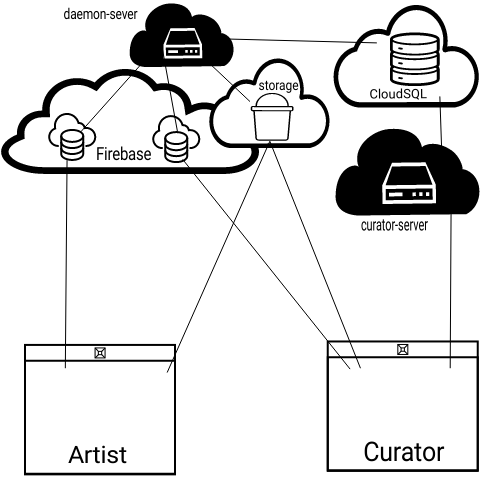
\includegraphics[scale=.5]{./img/tekuma-1}
    \caption{Arist-Curator System Diagram: (1) The daemon-server listens to the Firebase DBs and can insert into the SQL DB. (2) Firebase Databases hold all interface-state related data for both portals. (3) The storage bucket holds all of Tekuma's images, and acts as a CDN to the portals. (4) The curator-server mediates queries from the curator to the SQL DB.}
    \label{}
\end{figure}


\subsection{Boilerplate}
Before creating the web applications, a general boilerplate was designed for online user interfaces. The boilerplate makes up Tekuma's online graphic and visual identity. The UI primarily defaults to customs and principles dictated by Google's Material Design\footnote{\url{https://material.io/guidelines/}} in line with the current standards in User Interface design. Also included with the boilerplate is Tekuma's general CSS stylesheet, and a set of interface icons created by Afika Nyati. The style sheet builds upon the material design guidelines by customizing it to Tekuma's aesthetics. More technically, the interface is written in JavaScript ES6+ using ReactJS, transpiled using webpack and BabelJS. State in the interfaces, user account creation, and file uploads are all handled by Google Firebase and managed in the Firebase Conosole. For simplicity, all code in the system is written in JavaScript and is either executed in-browser, or with NodeJS (v6.4.0LTS). Together, the stylesheet, ReactJS interface components, logo, color palette and gradient, type choices (Nexa font, utf-8) makeup Tekuma's online visual identity, an extrapolation of Tekuma's brand identity developed by Kwaku Opoku in collaboration with Tekuma's founders.


\subsection{Artist}


The first component designed and implemented was the beta version of the Artist portal. The Artist portal is powered primarily by Google Firebase, and was originally designed to function without server-side code as a staticly served interface. All communications from the portal to the rest of the curation system are handled through the Firebase Realtime Database. The Artist Portal provides two main functionalities to its users, as well as a standard interface for editing and supplying personal information about themselves and their artistic style. The Artist portal has 833 accounts made (as of April 2017), with artists uploading 5571\footnote{ \url{https://docs.google.com/spreadsheets/d/1JO5Ouq5IeD7MJ87D-bqvoQoXAHpoKo89tOfHbUqqJbk}} total artworks since the beta release in July, 2016.\\




\subsubsection{Artist Studio}
The primary goal of the portal is to handle uploaded and cataloging of artworks. All uploaded files are saved into Google Cloud Storage buckets, located at in the Cloud Console\footnote{\url{https://console.cloud.google.com/storage/browser/art-uploads/?project=artist-tekuma-4a697}}, and all data cataloged in hierarchical (non-structural) format in the Firebase Database. The organization of these files within the storage buckets is detailed further in url-schema.md in the Documentation repositiory\footnote{ https://github.com/tekuma/documentation}. In the Studio, artists can organize their artworks into albums, edit the name and creator of the artwork, add or remove tag words, add a date of creation, as well as leave a description of the artwork. Whenever an artist is satisfied with the information supplied with the artwork, they can submit button (an up arrow) on the artwork tile. This will appear in the Curator app, explained in (2.4.3).
\begin{figure}
    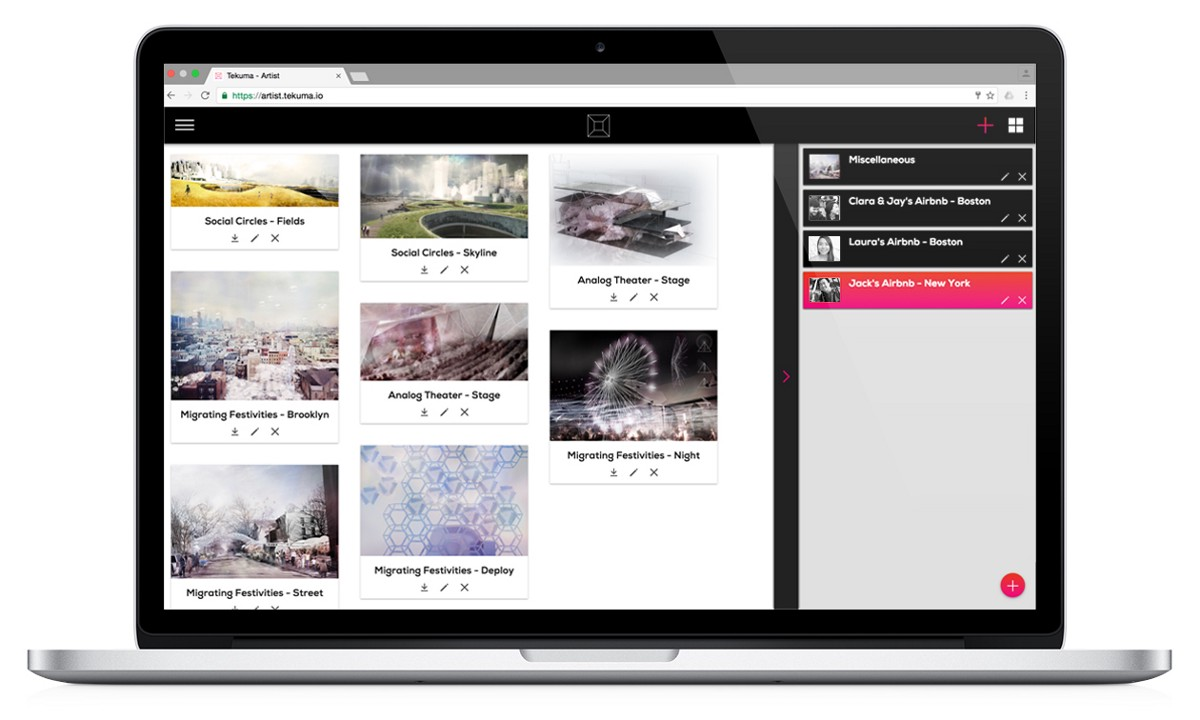
\includegraphics[scale=0.2]{./img/artist.jpg}
    \caption{The Artist Portal}
    \label{artist}
\end{figure}

\subsubsection{Artist Gallery}
The artist Gallery provides a list of all artworks which an artist has submitted to Tekuma. When one is clicked, more information appears, such as the review status (pending, approved, declined, or held), and any comments from the reviewing staff. Information that is reflected about the artwork here is what information is in Tekuma's database. Information such as sales data for that artwork can also be displayed here.

\subsubsection{Artist Admin Mode}
The Artist Portal also has an admin mode. This was explicitly created so that Tekuma Administrators can impersonate artsits and update/submit/change artwork details on their behalf. Which users are admins is explictly stated in the source code, and Firebase Database rules. Currently, only 4 accounts have this access.


\subsubsection{Artist Daemon}
Later, functionality was added to do extra processing on uploaded artworks to provide more labeled data. This functionality exceeded the scope of client-side execution, and integrating HTTP communication to a server would incure a large overhead. Instead, a daemon running on a Google Compute Engine (GCE) cloud-hosted server handles this extra processing. Communication to the daemon is facilitated by Google Firebase's real-time database where a first-in-first-out (FIFO) stack is used to keep track of jobs for the daemon to execute. Jobs added to the stack have different task fields for things like resizing an image, submitting an artwork, and tagging an image. The extra labeling includes gathering text tags and color palletes from the uploaded images using machine-vision technology via the Clarif.ai API\footnote{\url{https://www.clarifai.com/}}. The Artist Daemon also serves another purpose. Data about submitted/approved artworks is stored in the Curator's Firebase database. This prevents any artist from having write permission to their submissions. But since the artist can not write in order to submit an artwork, it sends a job to the Artist Daemon, and the daemon submits into the Curator's Firebase DB.

\subsection{Business}
The Tekuma Business portal has not yet been implemented.\\

\subsection{Curator}

The curator portal serves as a place where Tekuma's proprietary data (from the Artist Portal, or from partnerships) is stored. The curator portal also serves as an administrative portal for artworks submitted from the artist portal. The curator portal also has infrastructure to serve as an administrative system over the artist portal, by deciding what data is moved from the artist-portal database, into curator-portal's database.
The curator-portal's database serves as Tekuma's proprietary listing of curatable artwork, and therefore has more isolation than the artist-portal's database. Additionally, the curator database is an SQL database, served from a Google Cloud SQL instance running MySQL. The SQL database is more efficient for searches than the NoSQL structure used by Firebase.


\subsubsection{Curator Search}
\begin{figure}
    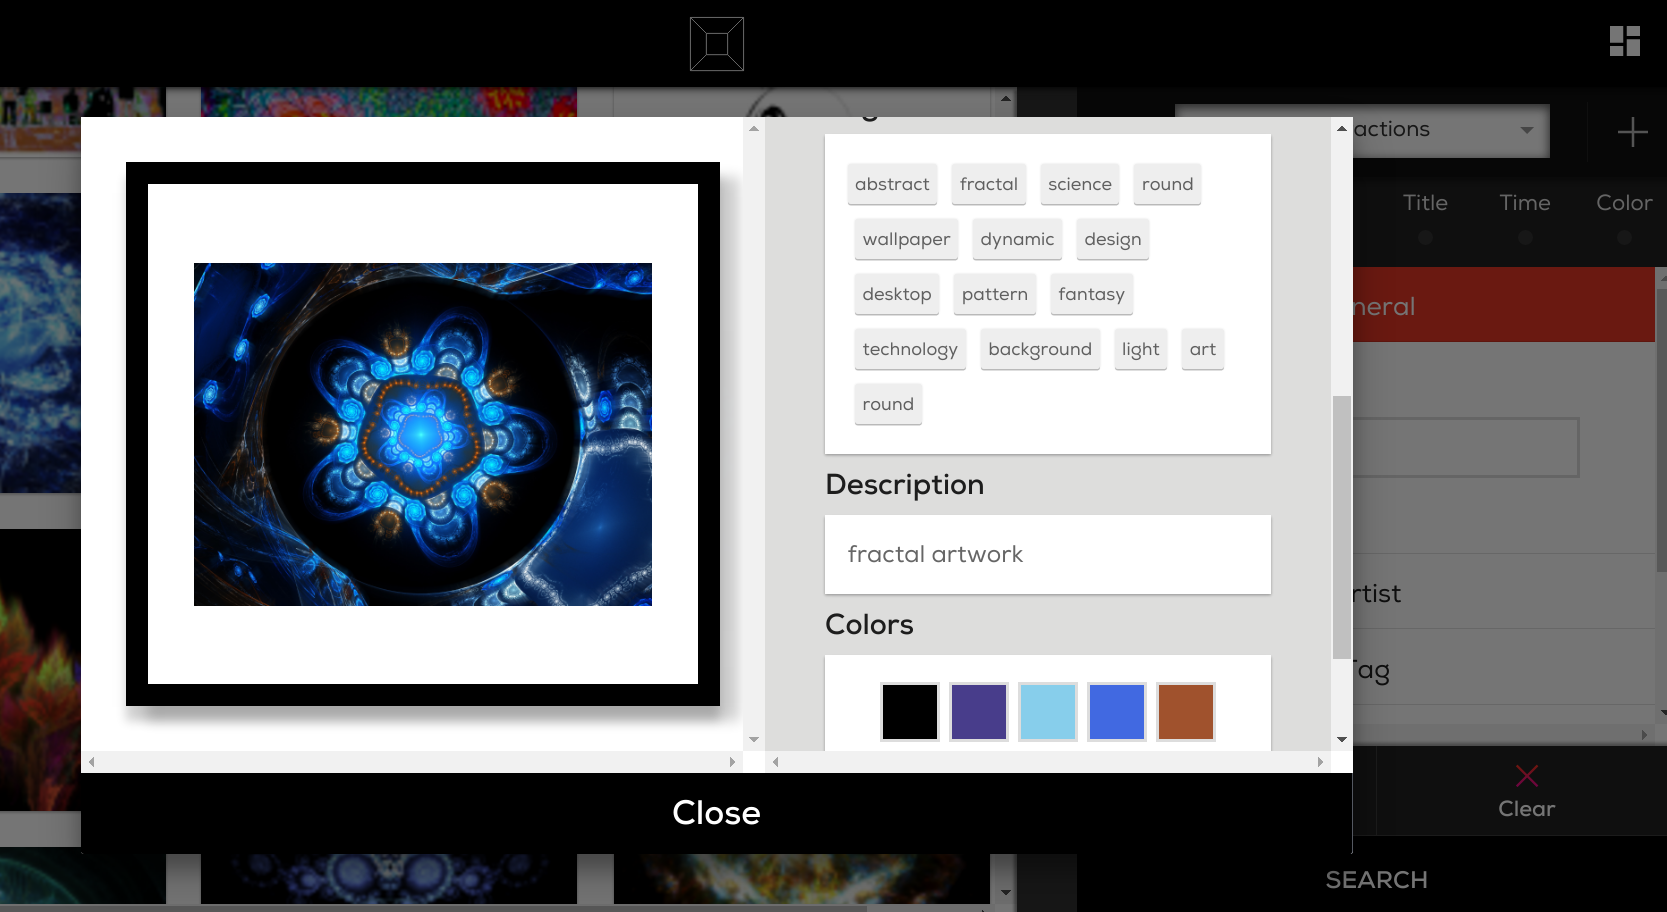
\includegraphics[scale=0.2]{./img/curator}
    \caption{Screenshot from the Curator Portal}
    \label{}
\end{figure}


The curator portal provides a very rich interface for queries which accepts words, colors, tag words, dates, and details about artists. In the figure on the right, full details about a search result are displayed. Notice the tag words, description field, and color palette associated with image.
Search results can then be added to a Project, in similar fashion to how you add items to a cart in an e-commerce user experience. Queries are sent from the interface to the curator-server\footnote{\url{https://console.cloud.google.com/compute/instancesDetail/zones/us-east1-c/instances/curator-tekuma-1}} via HTTPS (AJAX). The server then communicates the queries to the MySQL instance, and returns the result to the interface.  The server back-end uses an open-source solution (Node.js) and is served with nginx\footnote{\url{https://nginx.org/en/}}.

\subsubsection{Curator Manage}
These projects have their own interface, where curators can: share the project with other curators, leave notes and comments on the project, download images from the project, and export all data from the project in CSV format.

\subsubsection{Curator Review}
Curator's review interface acts an administrative interface over artworks submitted from the artist portal. Artworks enter as Submitted, and can be moved to: Declined, Approved, or Held.  Approved and Declined are terminal states, once the artwork is moved there it is either inserted into the SQL database, or deleted. Items moved to held allow the Artist to make changes to the information about the artwork, and re-submit it. Upon re-submitting, the artwork is removed the held branch and added to the Submitted branch again.

\subsubsection{Curator Daemon}
The Curator Daemon serves multiple functions. It acts as a user with access to both the Artist and Curator Firebase Database. First, when a Curator (in Review) moves an artwork into the 'held' branch, the daemon unlocks that artwork. This is because when an artist submits an artwork, it becomes locked since curators have been notified and the data needs to remain constant until the review.
The Curator Daemon is also responsible for inserting newly approved artworks into the SQL database. To do this, it establishes a connection to the MySQL server in Google Cloud, and forms a transaction for all of the artwork's relevant data, and executes the transaction. If they transaction was successful, the respective (with same artwork uid) artwork object in the Approved branch of the Curator Firebase DB with have a field of 'sql: true'.

\subsection{Discover}
The Discover Portal serves as the consumer-facing e-commerce store where arbitrary consumers can buy individual prints. The website is currently managed with a WordPress backend, using Shopify for handling e-commerce technologies. There is currently no proprietary infrastructure involved with the Discover Portal.

\section{Unfinished Components}
\subsection{Business}
No work on the business portal has been done. Conceptually, the business portal would use the same interface boilerplate as the artist and curator portals, and would allow for business users to have a dashboard of the properties with information the curation that is happening in these properties. Currently, the functionality of the business portal is handled by sales, and automation is not crucial.

\subsection{Discovery}
Eventually, data on the Discover portal from sales and product cataloging from Shopify (accessible via the Shopify API) should be connected a table in the SQL database. Currently, this data is kept separte from the existing infrastructure and is only accessible through scripts or user interfaces. Linking this data together would allow for more automation, and would allow sales figures to be reflected in the Artist Portal. Additionally, data should be collected on the Discover portal about which artworks each user likes, for later machine learning analysis.

\subsection{Testing Suite}
Test coverage for the deployed applications is low. Ideally, all production applications should have high code coverage, and an continious integration system should be implemented for deployments. Testing frameworks exist in both the Artist and Curator code bases, and TravisCI has been configured, but these components need further work.

\section{Databases}
\subsection{Arist Database}
Generally, the Firebase Databases are used to handle interface state. In the Artist Portal, it stores all the data for each user, including their information and uploaded artworks. To directly interact with the database, go to:\\
\url{https://console.firebase.google.com/project/artist-tekuma-4a697/database/data} \\
The database has 3 branches from root, \_private, jobs, and public. \_private and public then both have an onboarders branch, keyed by all artist UIDs. The jobs branch acts as the stack for the artist daemon.

Tekuma Art Database from artist.tekuma.io currently has 5571 artworks, uploaded from roughly 700 users. Rather than stored in rows/columns in relational SQL data, Artist portal data is stored in hierarchical, nested JSON storage that is used by Google Firebase. Each entry of this dataset contains (at some depth in the tree):
A description left by the artist
\begin{itemize}
    \item Artist Name
    \item Artwork Title
    \item Date of creation by artist
    \item Date of upload by artist
    \item Album Title of artwork
    \item Title (name) of the artwork
    \item size of the original upload
    \item Artwork UID a unique identifier in Tekuma's system
\end{itemize}
And, after additional processing from the image daemon, the following is also available ( on roughly 90\% of uploaded artworks):
\begin{itemize}
    \item A set of tags of nondeterministic size. E.g. \{“abstract”, “majestic”, “dog”, ”animal”\}
    \item A set of colors of nondeterministic size, constrained to length of 3-8. Each color saved has: \begin{itemize}
        \item A Hex value,  $\Rightarrow$ \#9fa29c
        \item A density or population in the image,  $\Rightarrow$ 0.608
        \item The closest color in the set of W3C’s list of named CSS colors\footnote{\url{https://www.w3schools.com/cssref/css_colors.asp }} $\Rightarrow$  \#a9a9a9/DarkGray
    \end{itemize}

\end{itemize}


\subsection{Curator Database}
The Curator Database holds all of the Curator's state data (like users, projects, etc). The Curator Firebase database also holds the 4 review branches submissions, held, approved, and declined. The Curator Firebase database can be accessed at : \\
\url{https://console.firebase.google.com/project/curator-tekuma/database/data}


\subsection{Tekuma Artwork DB}
The SQL database contains 6 tables, (artworks, artist, associations, locations, collections, labels). Each artwork has an entry in the artworks table, keyed by the artwork UID. Each row contains:
\begin{itemize}
    \item uid (char)
    \item title (char)
    \item description (text)
    \item artist\_uid (char)
    \item date\_of\_addition (DATETIME)
    \item date\_of\_creation (DATETIME)
    \item thumbnail\_url (char)
    \item origin (char)
    \item reverse\_lookup (char)
    \item META (blob)
\end{itemize}
More details can be found in the documentation repository.

\subsection{Art.com Database}
The Art.com Database, which is roughly 10MB, contains \textbf{2,311,390} rows of data, in structured SQL format. Examples of these rows are below.\\

\begin{lstlisting}[language=Python]
columns = [ 'SKU', 'ITEM_TITLE',  'ITEM_LONG_DESC',  'ARTISTNAME',    'ITEM_TYPE',  'IMAGE_URL',  'PRODUCT_URL', 'PRODUCT_TAXONOMY' ]
actual_row = [ '30742196502A',
  'Spurzheim Bust',
  'JOHANN KASPAR SPURZHEIM German phrenologist with his autograph',
  'H Corbould',
  'Photographic Print',
  'http://cache2.allpostersimages.com/MED/\\84\\8488\\5WQK300Z.jpg',
  'http://www.art.com/products/p30742196502-sa-i9032642/.htm?RFID=197560',
  'World Culture>European  Cultures>German Culture>>>>>>>' ]
\end{lstlisting}

\section{Related Work}
\begin{enumerate}
    \item\textbf{ArtFlip} (\url{https://www.artflip.com/product}) A website very similar in UI and UX to the curator portal.
    \item\textbf{Artsy}  (\url{https://www.artsy.net/collect})
    \item\textbf{Canvis} (\url{http://canviz.co/contact/})  A mass producible digital picture frame, including 3D printer files.
    \item\textbf{StitchFix} (\url{https://www.stitchfix.com/})  a clothing company which uses a mixture of expert human stylists and artificial intelligence to pick out outfits for customers on a subscription plan.
    \item\textbf{Turning Art} (\url{https://www.turningart.com/gallery}) A curator company with a similar buisness model of directed towards office, commericial, and multi-family real estate.
    \item\textbf{Large-scale Classification of Fine-Art Paintings} (\url{https://arxiv.org/pdf/1505.00855v1.pdf}) Details large scale classification algorithms for fine art paintings.
    \item\textbf{A Neural Algorithm of Artistic Style} (\url{https://arxiv.org/pdf/1508.06576.pdf}) Describes methods of transfering artist styles between artworks use Convolutional Neural Nets.
    \item\textbf{Inceptionism: Going Deeper into Neural Networks} (\url{https://research.googleblog.com/2015/06/inceptionism-going-deeper-into-neural.html}) Discussion of Google Deepdream
\end{enumerate}

\section{Potential Innovative Development Projects}
\subsection{Collaborative Art Recommender System}
 This section details methods which are \textit{agnostic} to the content. In other words, the AI is unaware that it is filtering artworks specifically. Collaborative filtering is currently a ubiquitous feature of internet based creative content platforms such as Spotify and Netflix. Collaborative filtering is commonly implemented with either data clustering, or low-rank matrix multiplication (better for sparse data), and relies on having a active user base. The underlying assumption of collaborative filtering is that if user (A) likes artworks {a,b,c,d} and user (B) likes artworks {a,b,c}, then it is likely he will also like artwork {d} as well. The strength of this method is that it is agnostic to the content, which is especially powerful for art and media, as it is inherently abstract and hard to break it down into concrete features.

\subsection{TekumAI, Curated Recommender System}
 This section details methods which are \textit{content-based}, meaning that the features of the artwork are directly considered by the system. This relies on the assumption that all artworks in the system have a concrete list of their features, known as a feature vector. Features in this vector have a numerical representation, and are chosen such that they partition the artworks into separate sets which people might conceivably assign different preferences to. Then, each user is assigned a user vector, $\theta$, which is continually updated to reflect the user's preferences. When this vector is initialized (usually with random values), it is not very powerful. This is known as the cold-start problem. Methods for circumventing cold start can "borrow" data from other places. Specifically, data could be borrowed from similar users, such as descbried in the previous section with collaborative filtering. The user could also be presented with a survey of his art tastes, which could be used to initialize the vector to something more accurate than if it was just set to random values. Given a feature vector $x^{(i)}$, we can predict a rating $\hat{y}$ by:
 $$ \hat{y}^{(i)} = \theta \cdot x^{(i)} = \sum_{j=1}^d \theta_jx^{(i)}_j $$
It is important to note that good features are those that partition the artworks into sets that people might
conceivably assign different preferences to. Data about the artist's personal story or description of the artwork can also be generated, possibly with a Bag of Words style implementation. Aside from cold start, another likely issue is not having enough good features. Additional features can be added by hand, or by artists, but this can also be automated. Methods for adding additional features using Convolutional Neural Nets is further explained in (5.6).\\
One possible user experience is to show the consumer an interface of artwork tiles, where swiping one way 'dislikes' an artwork, and swiping it the other way 'likes' it. Liked artworks can then be added to collections, and users can store these collections and buy prints from them.

\subsection{Artwork Meta-Search}
Similarly to how the curator portal provides an interface for curators to query for artworks, and sort them into projects, a meta search portal would do the same. Except, the meta-search portal would query many different online locations. One possible implementation is as follows:\\
\begin{enumerate}
    \item Use parts of the curator-portal interface as a boilerplate for making a similar interface for doing searches, and organizing results into projects.
    \item Configure a list of all relevant internet addresses which contain relevant artwork. This list would look something like: \begin{itemize}
        \item http://www.art.com/gallery/
        \item https://1x.com/photos/
        \item https://www.curioos.com/
        \item https://www.artflip.com/product/
        \item https://images.nga.gov/
    \end{itemize}
    \item Create a Google Custom Search Engine\footnote{\url{https://cse.google.com/cse/create }}, (CSE) and configure it to be an artwork search engine by listing artwork websites from (2).
    \item Create a back-end for the front-end interface which accepts queries. The back-end then can pass on that query string to a number of resources, and can return the results to the front end. Sources that the backend can query inculde: Tekuma's SQL database of art, the CSE mentioned above (via the JSON REST API\footnote{\url{https://developers.google.com/custom-search/json-api/v1/using_rest }}), and any partner APIs such as 1X.
    \item The server returns aggregated results from the above method to the frontend, similarly to the curator portal.

\end{enumerate}
\begin{figure}
    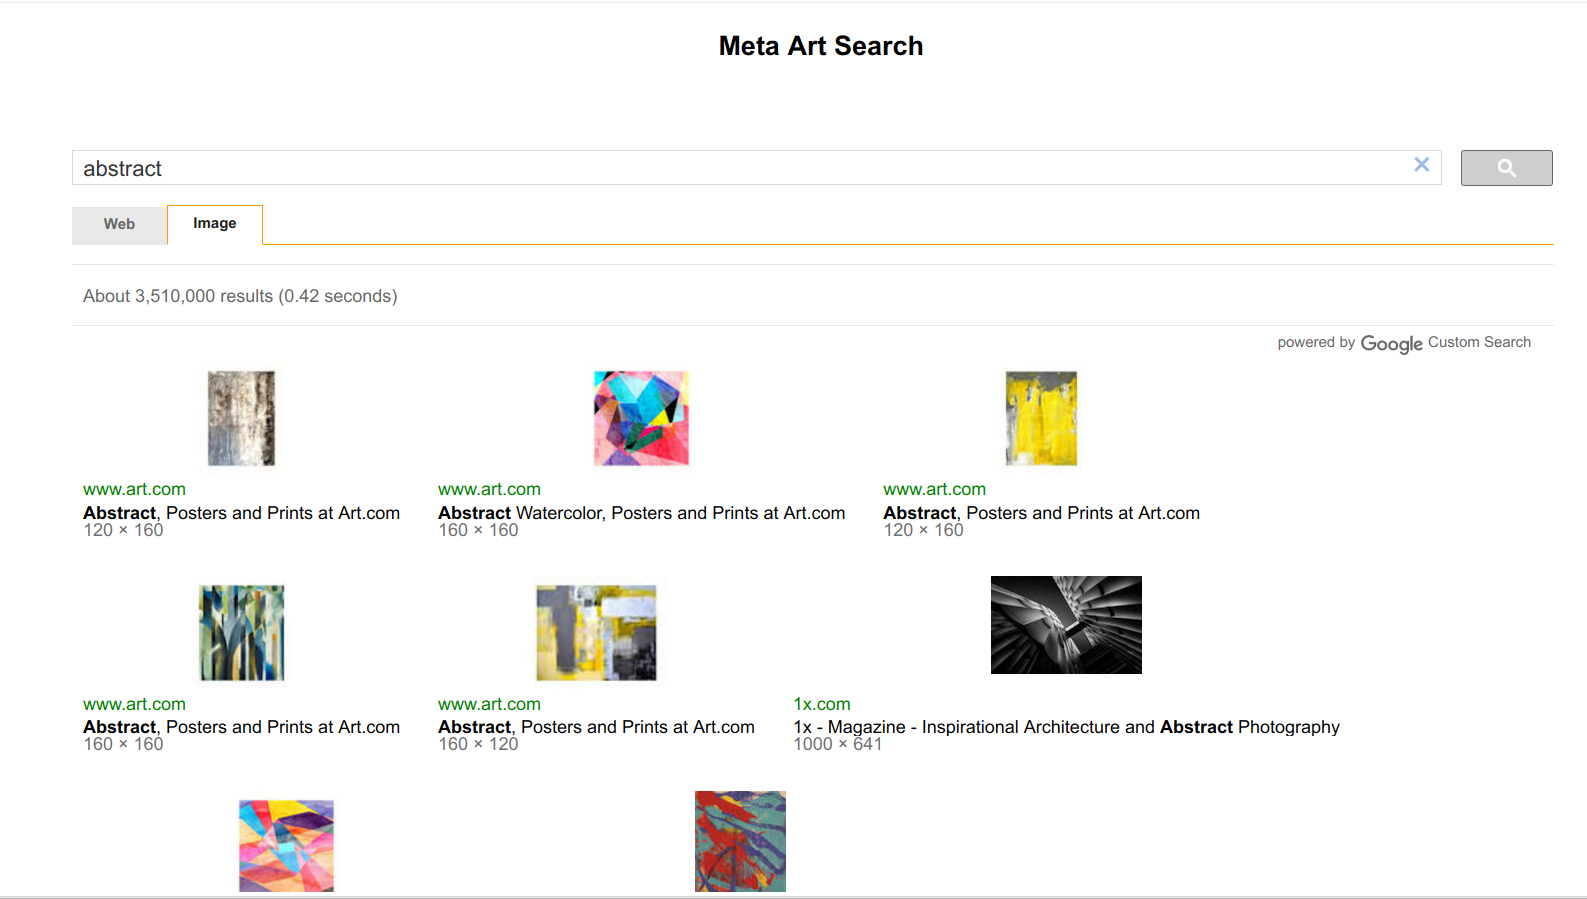
\includegraphics[scale=0.3]{./img/meta.png}
    \caption{Screenshot from a demo of a Google CSE with the list of sources}
    \label{meta}
\end{figure}

There are a few forseen issues with this implementation. First, this search functionality is not as rich as is possible in the curator portal. The CSE only searches text, and cannot detect other data such as color. Searches are also not restricted to individual artworks, and could return links to collections, artist pages, sales, or any other link inside the given domains. Results returned from the CSE API would need to be filtered with some sort of proprietary algorithm. Additional filtering from the CSE, as well as filtering or scraping on the server-side would need to be designed, tested, and implemented to effectively integrate this meta-search function.

\subsection{The Creative Social Network}
Existing infrastructure could be used to implement a social network between curators and artists. Artist submission, curator actions, etc could all be compiled to appear in a general newsfeed, where users could like/comment on stories which appear in the news feed, similarly to how existing social networks like Facebook and Instagram function. While the market here is decently saturated, other features could be implemented to innovate on creativity and make the network seem more attractive. For instance, a neural style-transfer feature could be added to the artist portal, using methods described in (5.7).  An artist could then, upload a work of their own and then have the option to have it “re-painted” in the style of Van Gogh, Picasso, or even a Tekuma featured artist like Decue Wu.  Additional ‘repainting’ features could also be used for more abstract art, such as DeepDream (5.8)  in which neural nets could be trained on different objects or patterns, and could alter the image to have more similar patterns to how the net was trained. This idea of a social creative platform also leads the way for Tekuma to provide a social platform for VR artwork.

\subsection{Cross-Media Recommendation}
Another interesting recommendation direction to explore, that to our best knowledge has yet to be implemented, is a recommendation system that recommends selected works from one medium based on the characteristics of a different medium. For example, using selected music catalogs or written media, such as poetry, to recommend (curate) a set of visual artworks. With regards to the choice of recommendation media, the most feasible choices would be those that are text-based, such as poems, or aurally-based, such as music.

\subsection{Interactive Art Gallery Experience}
An interactive gallery experience can be described as having a gallery in which patrons can interact with the artwork to learn more about it and its artist using technology. The simplest way to do this would be for patrons to use their phones as an interface to the artwork, with mobile apps or a web app. The difficult part is knowing which artwork the patron is standing in front of. There are a number of possible ways to engineer a solution:
\begin{enumerate}
    \item GPS/WiFi: the standard way your phone calculates location. Is highly reliable, but does not provide good accuracy indoors.
    \item Stylized QR codes. QR codes are still in wide use, and expanding in popularity in some areas. QR codes offer 100\% success on knowing which artwork the patron is standing at, but requires them to use a QR scanner each time.
    \item WiFi location sensing. Implementations such as SpotFi\footnote{\url{http://web.stanford.edu/~skatti/pubs/sigcomm15-spotfi.pdf}}, use commodity routers to guess the location of devices connected to routers. Great success has been had recently, and they can be accurate to 40cm even through walls, using open source solutions\footnote{\url{https://www.internalpositioning.com/}, \url{https://github.com/schollz/find}}.
\end{enumerate}

One of these methods described above could be implemented to provide localization to the interactive gallery experience. After localization is achieved, numerous features could be added such as:
\begin{enumerate}
    \item 3-D gallery of other artworks by that artist. Using three.js, a 3d room could be modeled, and users could pan their phones around to see in other directions, similar to a 3D video on facebook.
    \item More information the artwork and author can be displayed
    \item Sales information and a link to buy the artwork can be displayed
    \item Some sort of tailored AR experience mixing the location localization, phone, phone camera, and artwork could be devised. Perhaps this could be a model for AR art or "ARt"
\end{enumerate}

\section{Conclusion}
In summary, the foundation of Tekuma's platform and computer system have been set. Cloud computation has allowed for no physical servers to be used, and all servers, storage buckets, and databases are located in Google Cloud Console. Current operational costs are minimal, and the plaform is designed to scale. While a testing suite should be implemented to ensure the stablility of the system, and an audit of security (passwords, keys, accounts, etc) should be done before any further expansions, the platform is ready for more inovative applications to build upon it.

\end{document}
